\chapter{Resultados Experimentais}\label{chp:resultados}

Este capítulo discorre sobre os procedimentos realizados para a obtenção dos resultados comparativos da rmM-tree proposta por \citet{paper-fully-functinal-succint-trees},
com a rmM-tree k-ária proposta neste trabalho. Ele está dividido da seguinte forma: a Seção ~\ref{sec:base-de-dados} apresenta o conjunto de dados usado na avaliação experimental.
As seções seguintes apresentam as configurações da máquina usada para realizar os testes (Seção~\ref{sec:configuracao}), a metodologia usada (Seção~\ref{sec:experimentos}), e por último os resultados obtidos (Seção~\ref{sec:resultados}).


\section{Base de dados}\label{sec:base-de-dados}
Afim de realizar testes que comprovem o desempenho das estruturas implementadas na prática, usamos em nossos testes quatro conjuntos de dados do mundo real, estes conjuntos são apresentados em \citet{datasets-inf-udec}.
A Tabela~\ref{tbl:dataset} mostra um resumo dos conjuntos usados: a primeira coluna da tabela refere-se ao nome do conjunto de dados, a segunda coluna indica o tamanho do conjunto de dados em MB, a coluna de número 3 mostra a quantidade de parênteses do respectivo conjunto de dados, e por fim, a quarta coluna exibe a quantidade de nós da árvore representada pela sequência de parênteses balanceados.


\begin{table}[h!]
  \centering
  \caption[Conjunto de dados usados em testes experimetais]{Conjunto de dados usados nos testes experimetais }
  \label{tbl:dataset}
	\resizebox{\columnwidth}{!}{
        \begin{tabular}{|l|l|l|l|l|}
        \hline
        \textbf{Conjunto de dados}                       & \textbf{Tamanho (MB)}                      & \textbf{Quantidade de parênteses}                      & \textbf{Tamanho da árvore representada}  \\ \hline
        Complete tree (ctree)                            & 18                                          & 2.147.483.644                                          & 1.073.741.822                           \\ \hline
        DNA                                              & 135                                         & 1.154.482.174                                          & 577.241.087                             \\ \hline
        Proteins (prot)                                  & 82                                          & 670.721.006                                            & 335.36203                               \\ \hline
        Wikipedia   (wiki)                               & 13                                          & 498.753.914                                            & 249.376.957                             \\ \hline
        \end{tabular}
    }
\end{table}

Conforme é mostrado em \citet{datasets-inf-udec}, o  conjunto \textit{Complete tree} represeta uma árvore binária completa de profundidade igual à 30, ao passo que as sequências  de parênteses balanceados $DNA$/$Proteins$ representam uma árvore de sufixos de DNA e proteínas, respectivamente. Por último o conjunto \textit{Wikipedia} representa o XML extraído da Wikipédia no dia 12 de janeiro de 2015 \citep{datasets-inf-udec}.

\section{Configuração}\label{sec:configuracao}
Para realizar os testes de validação e de comparação de desempenho foi utilizado o servidor Turing, disponível no IFB. A máquina usada possui as seguintes configurações:
\begin{itemize}
    \item Arquitetura: x86;
    \item Processador: Intel Xeon Gold 5120;
    \item Frequência base: 2,20GHz;
    \item Frequência máxima: 3,20 GHz;
    \item Threads por core: 2;
    \item Cores: 28;
    \item Cache L1: 896 KiB;
    \item Cache L2: 28 MiB;
    \item Cache L3: 38.5 MiB;
    \item Memória RAM total: 527,03 Gb;
\end{itemize}

\section{Experimentos}\label{sec:experimentos}
\subsection{Decisões de projeto}\label{subsec:decision}
Os conjuntos mostrados acima fornecem árvores gerais no formato de parênteses balanceados, de modo que foi preciso pré-processar os conjuntos antes da execução dos testes, afim de adaptá-los à estrutura de vetores de bits, que serviu como base para a construção das range min-Max tree.

Para realizarmos uma comparação justa entre a estrutura proposta por \citet{paper-fully-functinal-succint-trees} e a estrutura proposta neste trabalho,  implementamos a rmM-tree no seu formato binário seguindo a descrição de \citet{book-compact-data-structures}. Após a implementação e validação dessa estrutura em seu formato binário, iniciamos a construção e validação da rmM-tree k-ária. Ambas as estruturas estão disponíveis no repositório \href{https://github.com/DanyelleAngelo/rmm-tree}{github.com/DanyelleAngelo/rmm-tree}, usando a linguagem de programação \textit{C++} e a biblioteca \textit{SDSL}. 

Durante os testes de desempenho (descritos com mais detalhes na Seção ~\ref{sec:benchmark}), fizemos algumas adaptações na nossa proposta, assim implementamos duas versões da rmM-tree k-ária, estas se diferem unicamente pelo processo de subida na árvore. A primeira versão (adotada neste trabalho), segue a abordagem de verificação dos irmãos à direita  (ou à esquerda, dependendo do sentido da busca) de um nó $v$, durante o percurso em árvore, como descrito por \citet{book-compact-data-structures}, para esta versão, o pior caso é observado durante uma busca iniciada em um nó $v$, com o excesso desejado não estando compreendido entre os registros dos irmãos de $v$, e $v$ sendo um dos primeiros filhos de seu nó pai. Buscando evitar este caso, construímos uma versão alternativa da rmM-tree k-ária, que não faz uso da técnica de visitação dos nós vizinhos proposta por \citet{book-compact-data-structures}, nesta versão ao terminarmos de inspecionar os registros de um nó $v$, avançamos na rmM-tree através do seu nó pai, verificando os registros deste nó, e inspecionando os demais filhos deste, apenas se a resposta estiver compreendida entre os registro de $v$.   

Outra importante decisão no projeto das nossas estruturas e que melhorou significativamente o seu desempenho, foi a implementação da função \textit{bitsread} como é exposto na Seção ~\ref{sec:sec-classic-rmm-tree}. Inicialmente essa função lia de modo iterativo $w-1$ bits a partir de um índice $i$, e realizava então uma pesquisa na tabela \textit{C} pelo elemento correspondente aos bits lidos, obtendo assim os valores de excesso necessários para a computação de diversas operações. Essa leitura iterativa acrescentava um tempo considerável às nossas operações. Substituímos então esse processo iterativo, por um processo usando operações de deslocamento de bits, inserimos também em nosso projeto o uso de uma tabela de reversão, para que pudessemos realizar a leitura dos bits, usando como critério de ínicio, o bit mais significativo da palavra.

\subsection{Testes unitários}
Objetivando garantir a asserção das respostas retornadas pela estrutura da rmM-tree binária e k-ária, realizamos a cada implementação -- e alteração  -- testes unitários usando o framework Google Tests.

No ínicio do desenvolvimento de cada estrutura foram criados testes com árvores gerais pequenas, comparamos os resultados da nossa implementação da rmM-tree binária, com os resultados da rmM-tree implementada na biblioteca \textit{Succint Data Structure Library} (SDSL), disponiblizada por \citet{sdsl}. Para algumas operações foi necessário computar o valor de retorno esperado usando uma série de operações básicas de vetores de bits, tendo em vista  que a SDSL não fornecia todas as operações necessárias para os testes de validação da nossa estrutura.

Após os primeiros testes de unidade, expandimos o nosso escopo de testes. Utilizando a sequência de parênteses \textit{Wikipedia}, geramos diversas consultas aleatórias afim de testar as operações da estrutura k-ária frente a estrutura binária.

No caso das operações que requeriam que o parâmetro de entrada correspondesse à um parênteses de abertura "(" ou de fechamento ")", foram pré-processados de modo aleatório os índices que atendiam a especificação, afim de realizarmos testes com entradas válidas.

\subsection{Testes de Desempenho}\label{sec:benchmark}
Após a construção de cada estrutura e tendo concluído os testes de validação, iniciamos os testes de desempenho, para tanto foi usado o framework Google Benchmark. Durante esses testes, foram introduzidas as melhorias citadas na Seção~\ref{subsec:decision}, sendo que à cada nova alteração, realizavamos novamente, todos os testes unitários, e testes de desempenho, afim de garantir a asserção dos nossos resultados.

Para os testes de desempenho, foram pré-computados diversos vetores pseudo-aleatórios, usando diferentes sementes (afim de manter uma variedade maior dos parâmetros usados), para diferentes operações. Cada um desses vetores tinham como entrada  índices dos conjuntos de dados usados nos testes, que caracterizam parâmetros válidos para as operações sobre as rmM-tree implementadas. 

Para cada operação foi usado cerca de $3.000.000$ de dados, os resultados de desempenho das mesmas é mostrado na próxima seção.

\section{Resultados}\label{sec:resultados}
O tempo gasto por cada operação da rmM-tree binária e k-ária sobre os conjuntos de dados citados, foi exportado para um arquivo \textit{.csv}, e a partir destes resultados, foram gerados gráficos de tempo médio gasto por cada operação, através da linguagem de programação Python. Estes gráficos são mostrados nas Figuras~\ref{fig:cstree}, \ref{fig:dna}, \ref{fig:prot} e \figref{fig:wiki}.

Os gráficos de barras aninhadas, agrupam os resultados para cada tipo de árvore por operação. As árvores geradas para os testes são:
\begin{itemize}
  \item rmM-tree binária (barra azul);
  \item rmM-tree 4-ária (barra laranja);
  \item rmM-tree 8-ária (barra verde), e
  \item rmM-tree 16-ária (barra vermelha).
\end{itemize}

 O tamanho de bloco usado em todos os testes foi definido como $32$, e a constante $w$ que divide $b$, foi setada como $16$, mantendo assim a tabela C, que auxilia na montagem da árvore e na verificação dos dados em cache.

O eixo $y$ dos nossos gráficos se refere ao tempo médio para $3.000.000$ consultas sobre as diferentes versões da rmM-tree, no eixo $x$ podemos ver os tipos de árvores comparadas, bem como as operações realizadas. 

Ressalta-se novamente que as operações \textit{minExcess, minSelectExcess, minCount} e suas derivadas não foram implementadas na nossa versão k-ária da rmM-tree, e por isso o desempenho das mesmas não foram levados em consideração pela nossa análise, além destas também não realizamos testes de benchmark para as operações que derivam exclusivamente de operações de acesso ao vetor que representa a árvore de entrada.

Como pode ser observado nos gráficos, a rmM-tree binária obteve melhor desempenho para todas as operações, isso está relacionado ao fato de que a rmM-tree binária, possui uma série de otimizações a nível de código, que não são implementadas na rmM-tree k-ária. Por exemplo, para a rmM-tree binária, o percurso em árvore é interrompido sempre que atingimos o último nó de um nível (ou primeiro de um nível, para o caso da operação \textit{bwdSearch}).

Além disso, o hardware utilizado possui uma cache relativamente grande em comparação aos conjuntos de dados analisados, desta forma os dados tendem a residir sempre em cache, inviabilizando a análise comparativa dos resultados encontrados pela rmM-tree binária e k-ária, haja vista que esta última deveria apresentar melhor resultado quando obtém uso otimizado da cache frente a estrutura original. 

Para as aridades da rmM-tree k-ária analisadas, não foi possível detectar um padrão para os diferentes conjuntos de dados. No geral, o desempenho das estruturas \textit{k-árias} variam entre si, para cada operação em unidades de \textit{nanossegundos}. 

Com base no conteúdo abordado neste trabalho, acredita-se que mediante à implementação de otimizações no código da rmM-tree k-ária, poderemos atingir o equilíbrio entre a quantidade de instruções executadas, e acessos a memória principal, melhorando assim o desempenho do sistema. Acredita-se também que a estrutura proposta mostrará seu potencial diante de um hardware mais modesto.

\newpage

\begin{figure}[!ht]
    \centering
      \caption[Operações sobre o conjunto de dado ctree]{Tempo médio de operações sobre o conjunto Complete Tree}{
          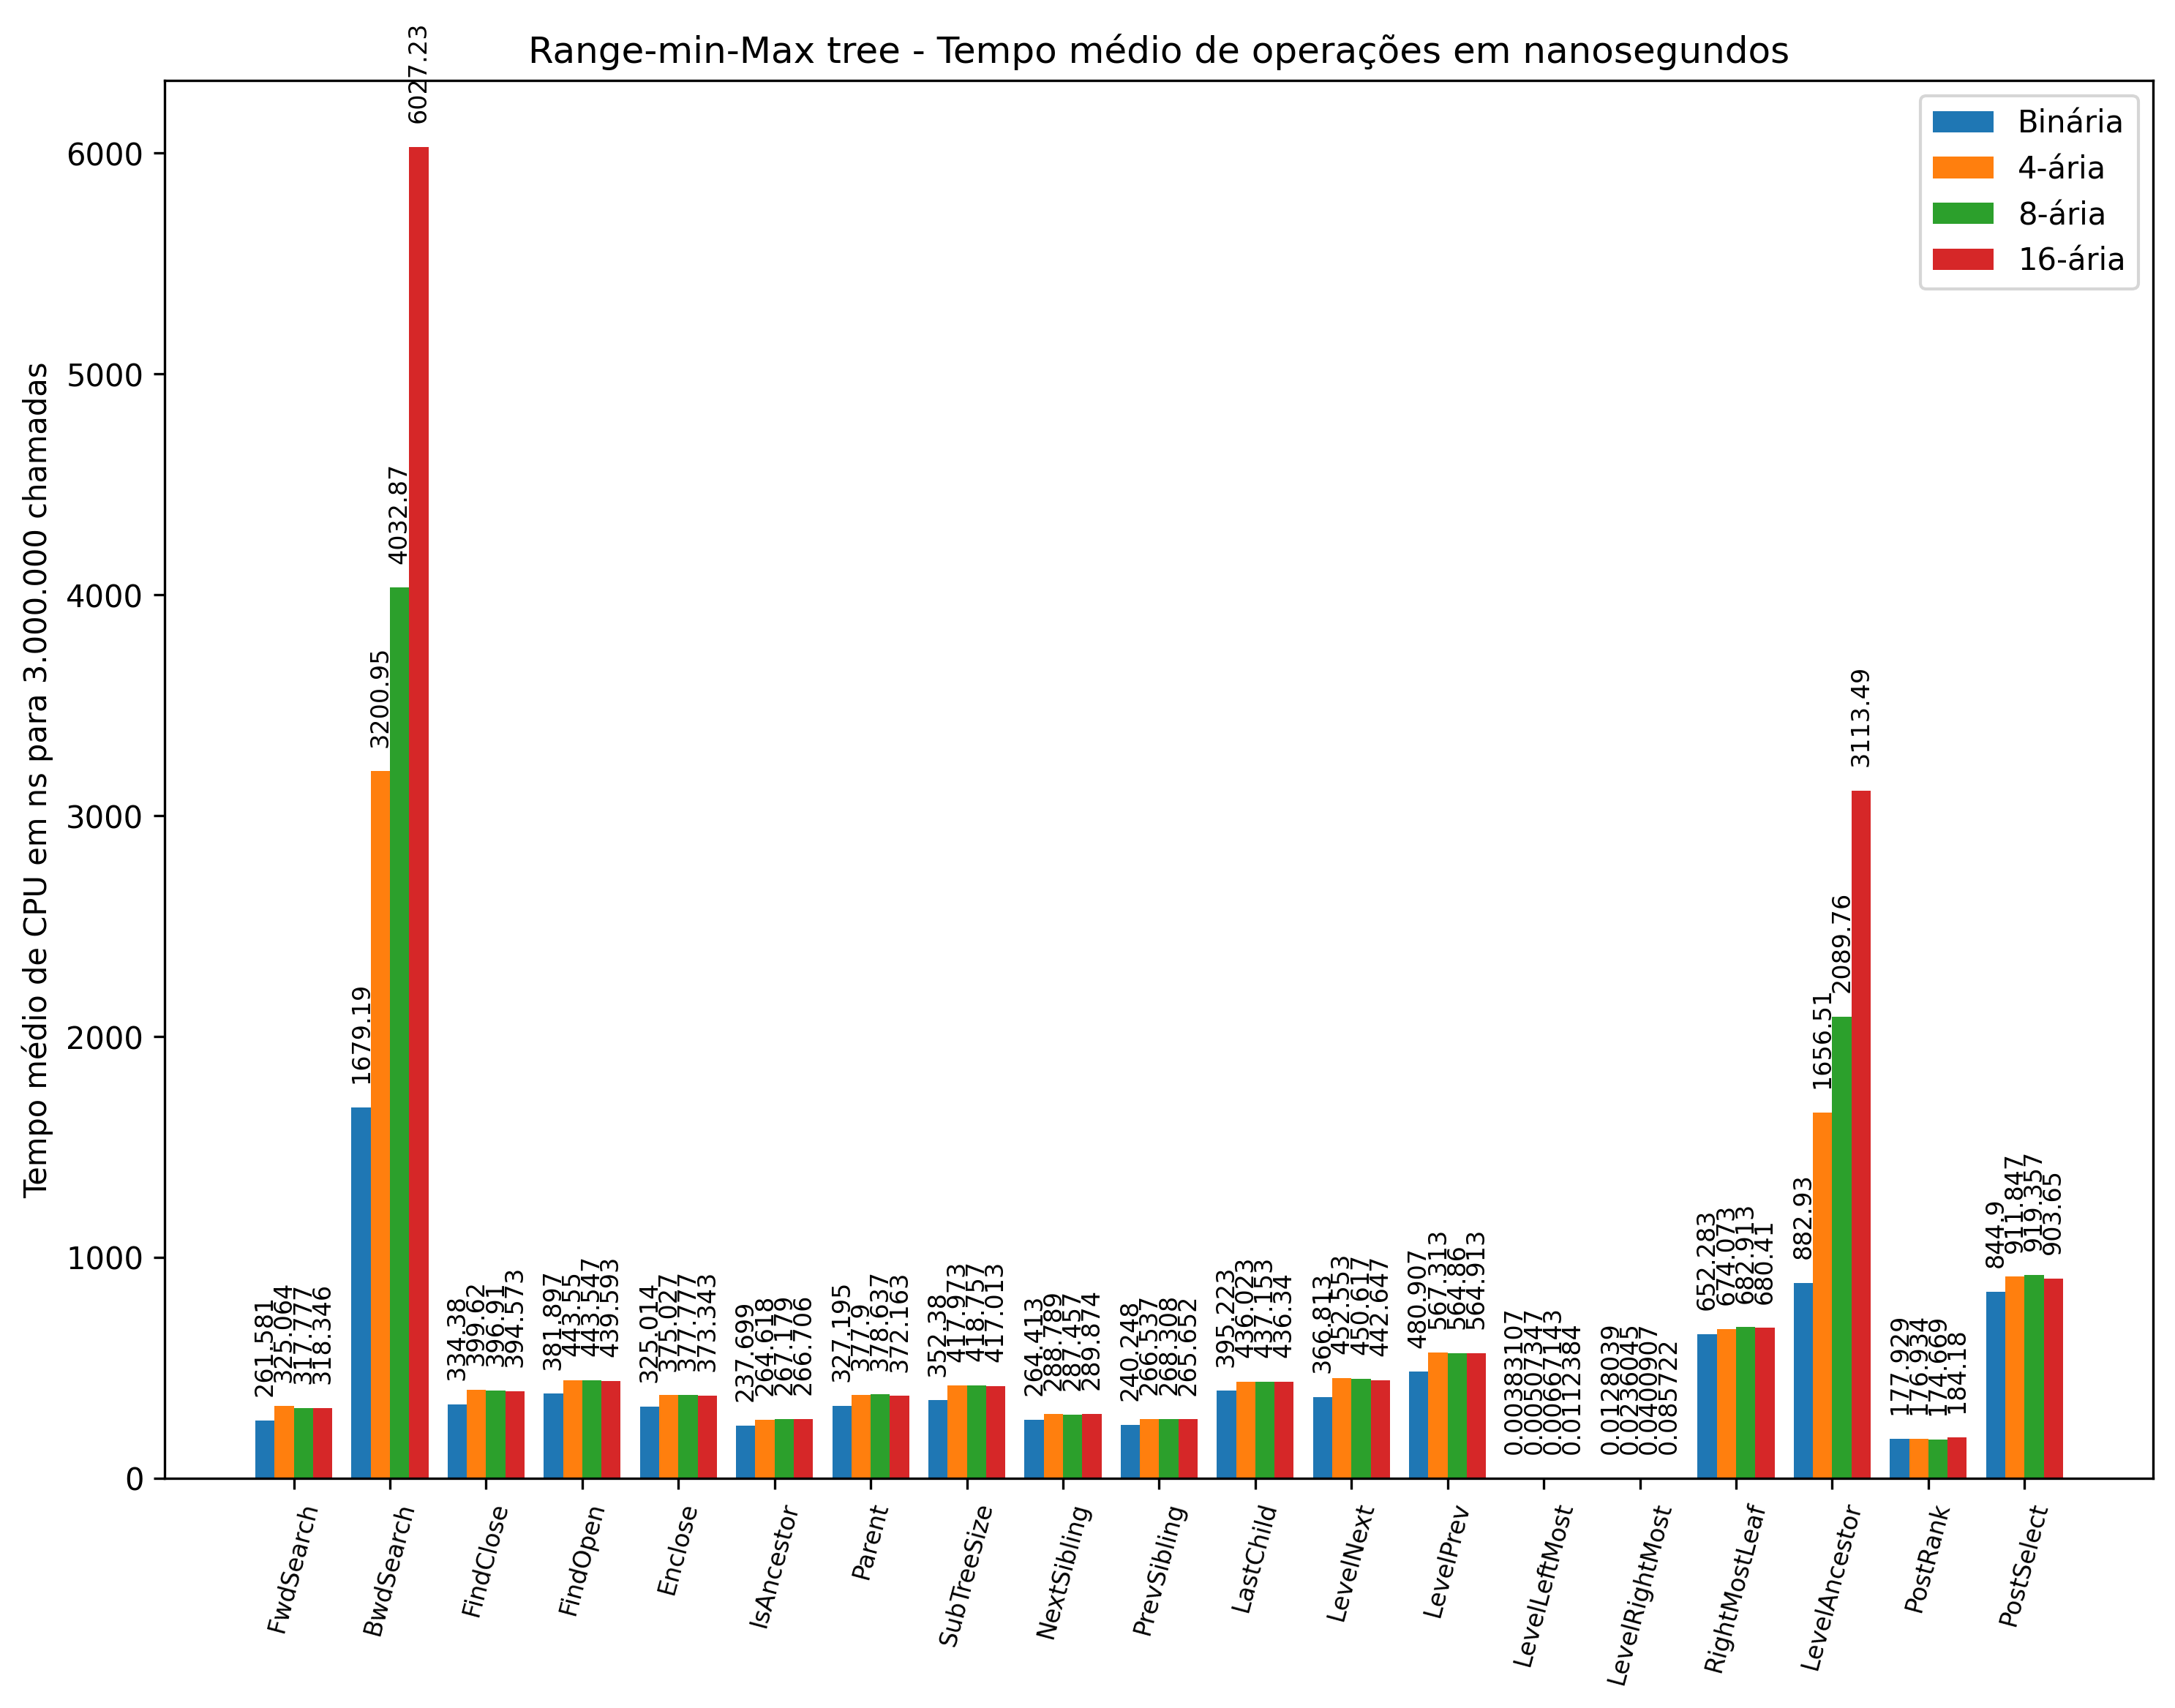
\includegraphics[scale=0.8, angle=270]{images/ctree_i3000000.png}
        }
        \label{fig:cstree}
\end{figure}

\begin{figure}[!ht]
    \centering
      \caption[Operações sobre o conjunto de dado dna]{Tempo médio de operações sobre o conjunto DNA}{
          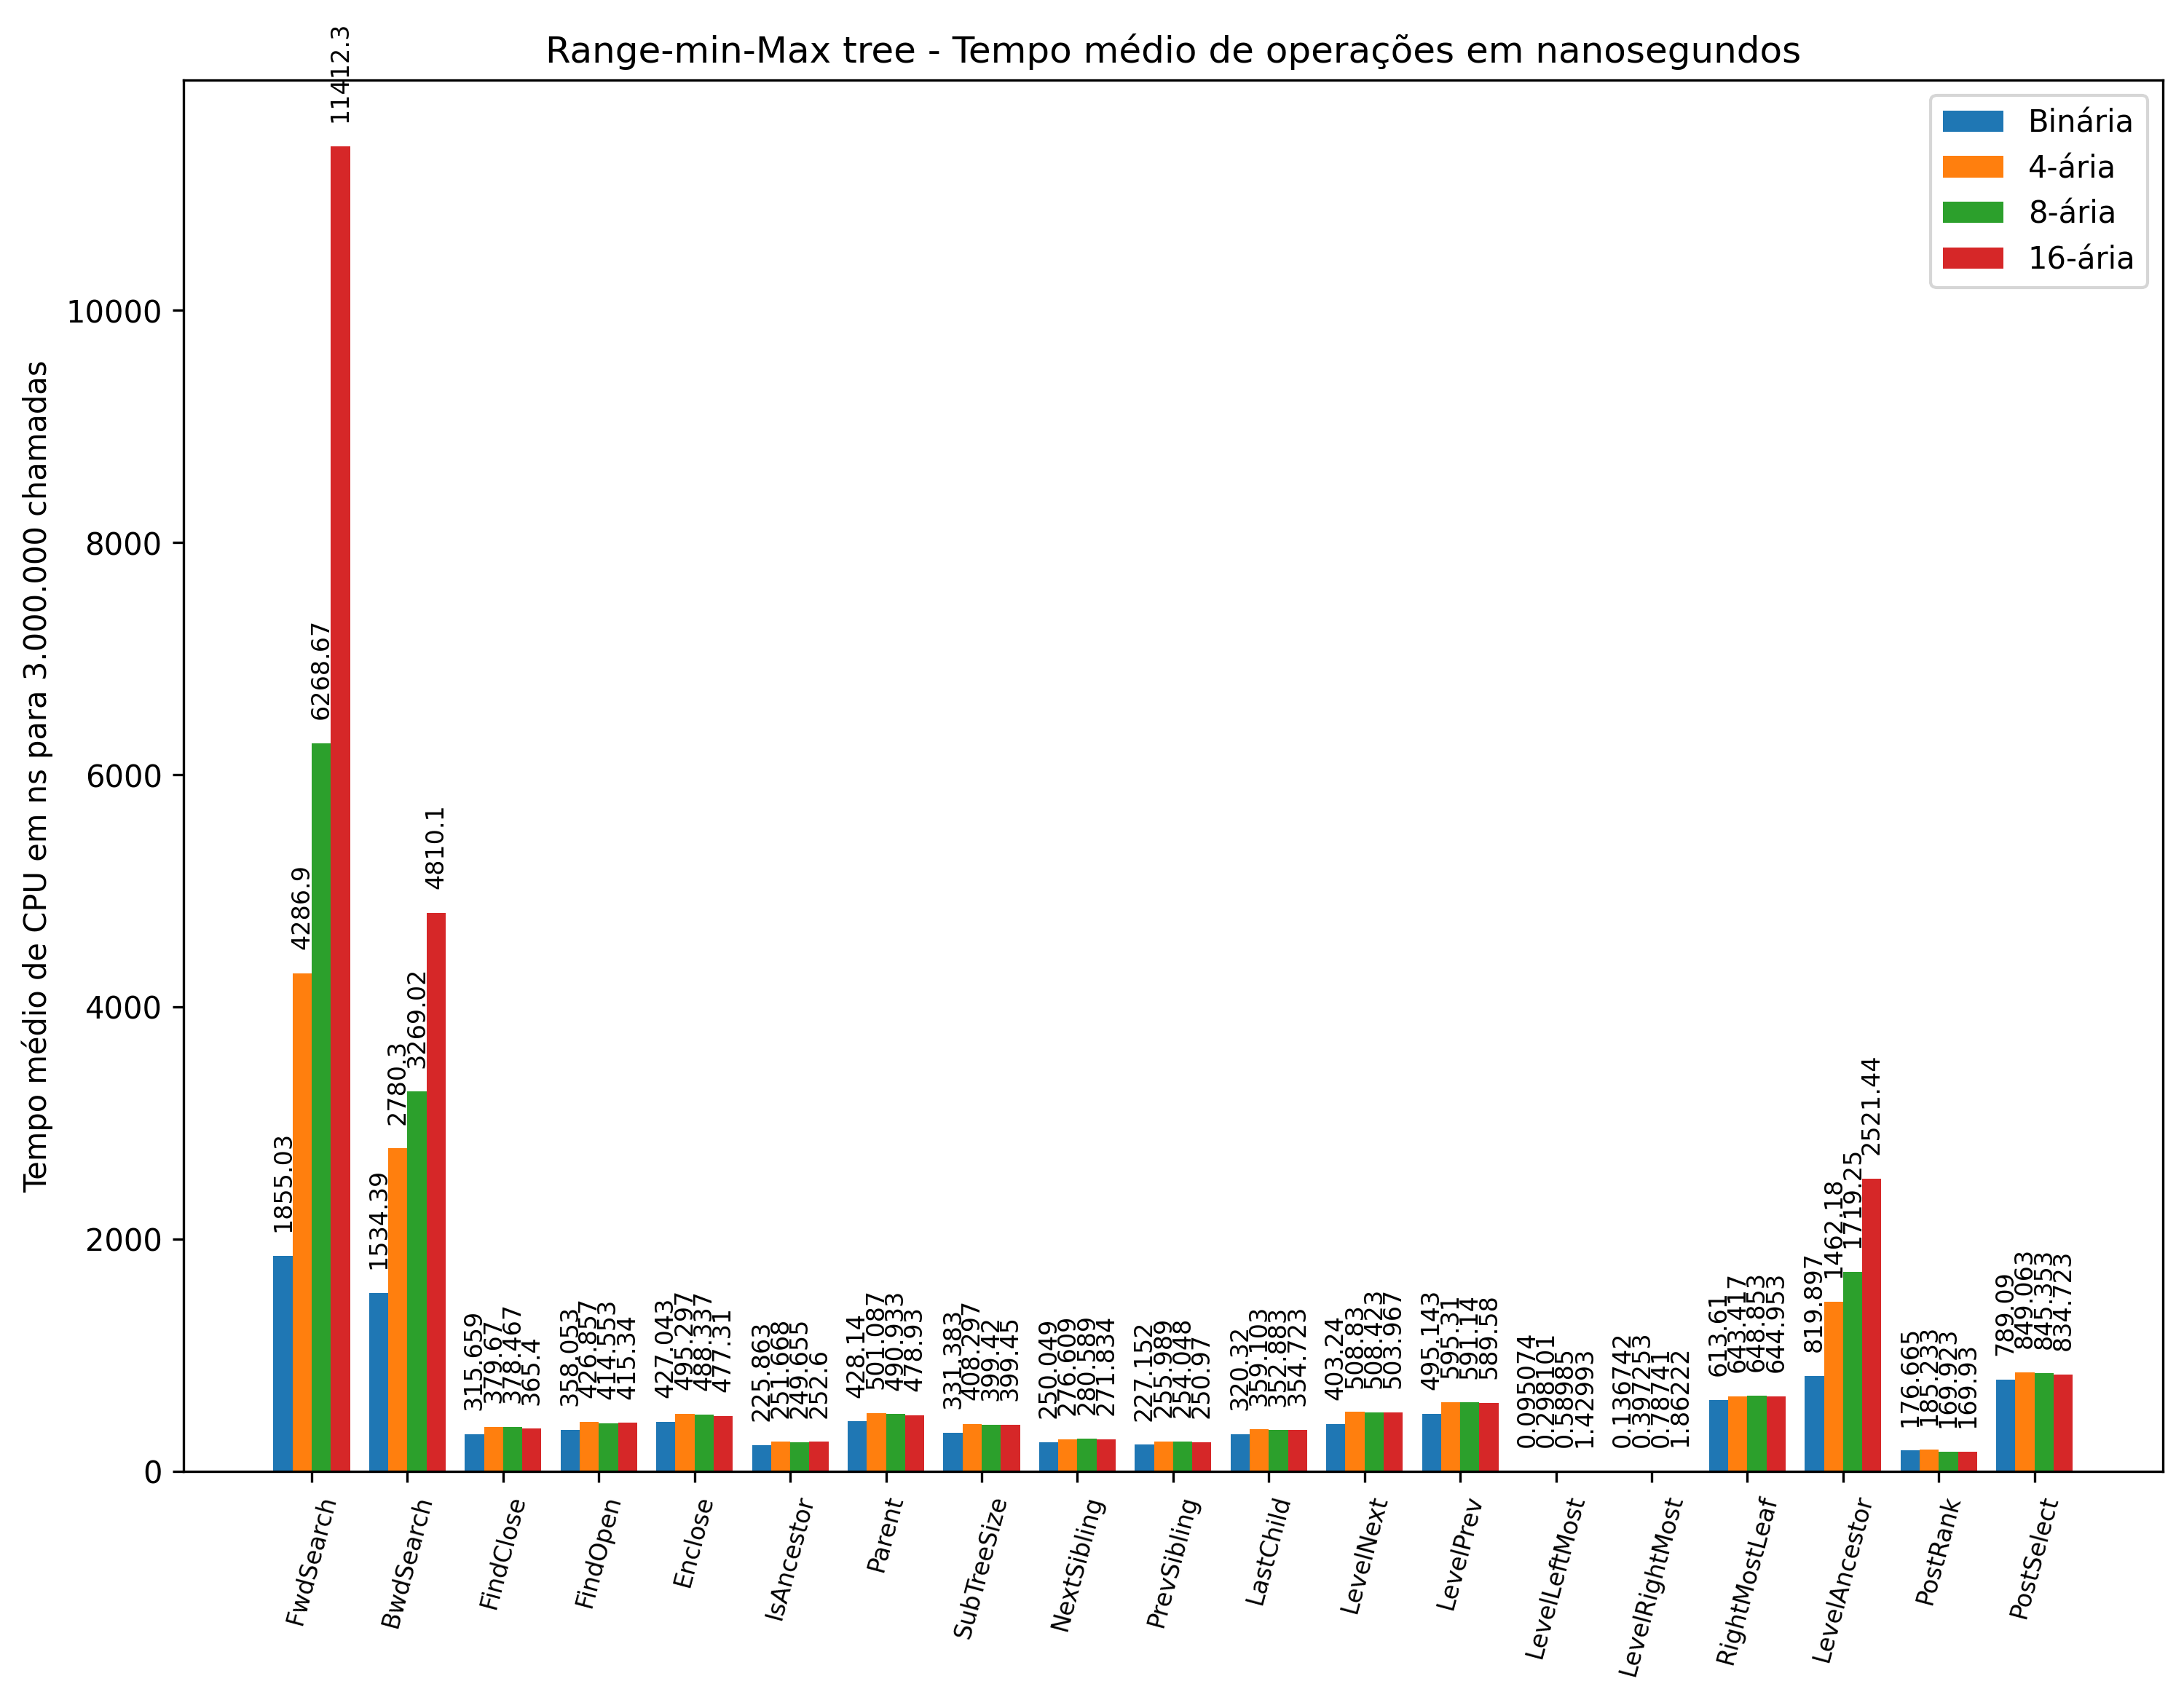
\includegraphics[scale=0.8, angle=270]{images/dna_i3000000.png}
        }
        \label{fig:dna}
\end{figure}

\begin{figure}[!ht]
    \centering
      \caption[Operações sobre o conjunto de dado proteins]{Tempo médio de operações sobre o conjunto Proteins}{
          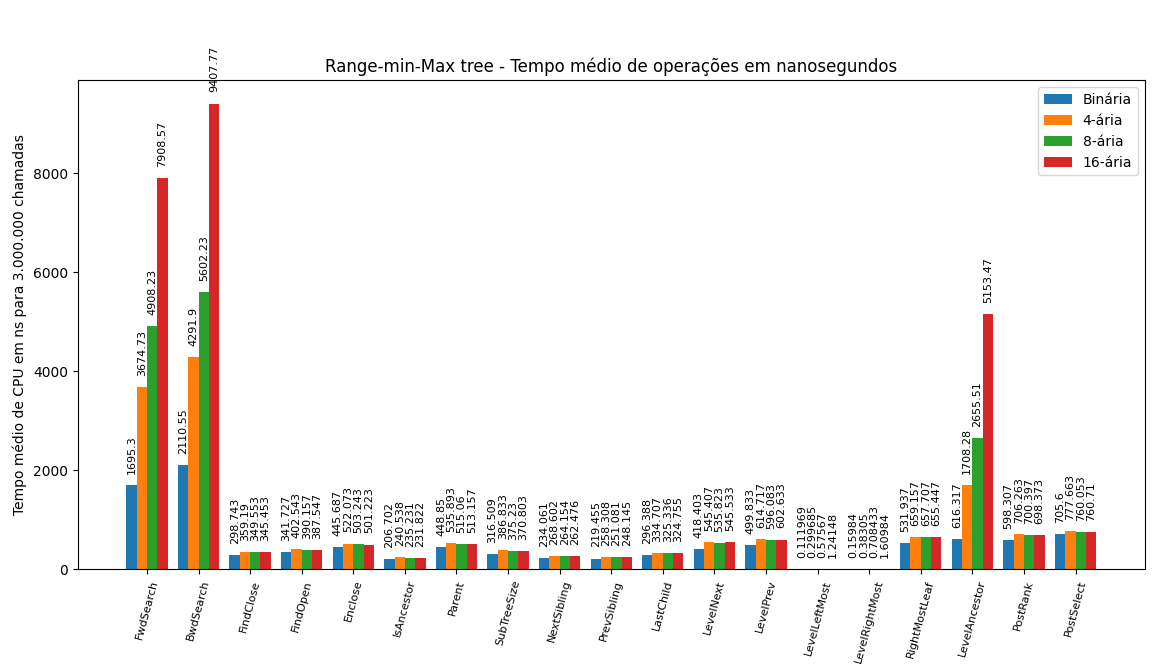
\includegraphics[scale=0.8, angle=270]{images/prot_i3000000.png}
        }
        \label{fig:prot}
\end{figure}

\begin{figure}[!ht]
    \centering
      \caption[Operações sobre o conjunto de dado wikipedia]{Tempo médio de operações sobre o conjunto Wikipedia}{
          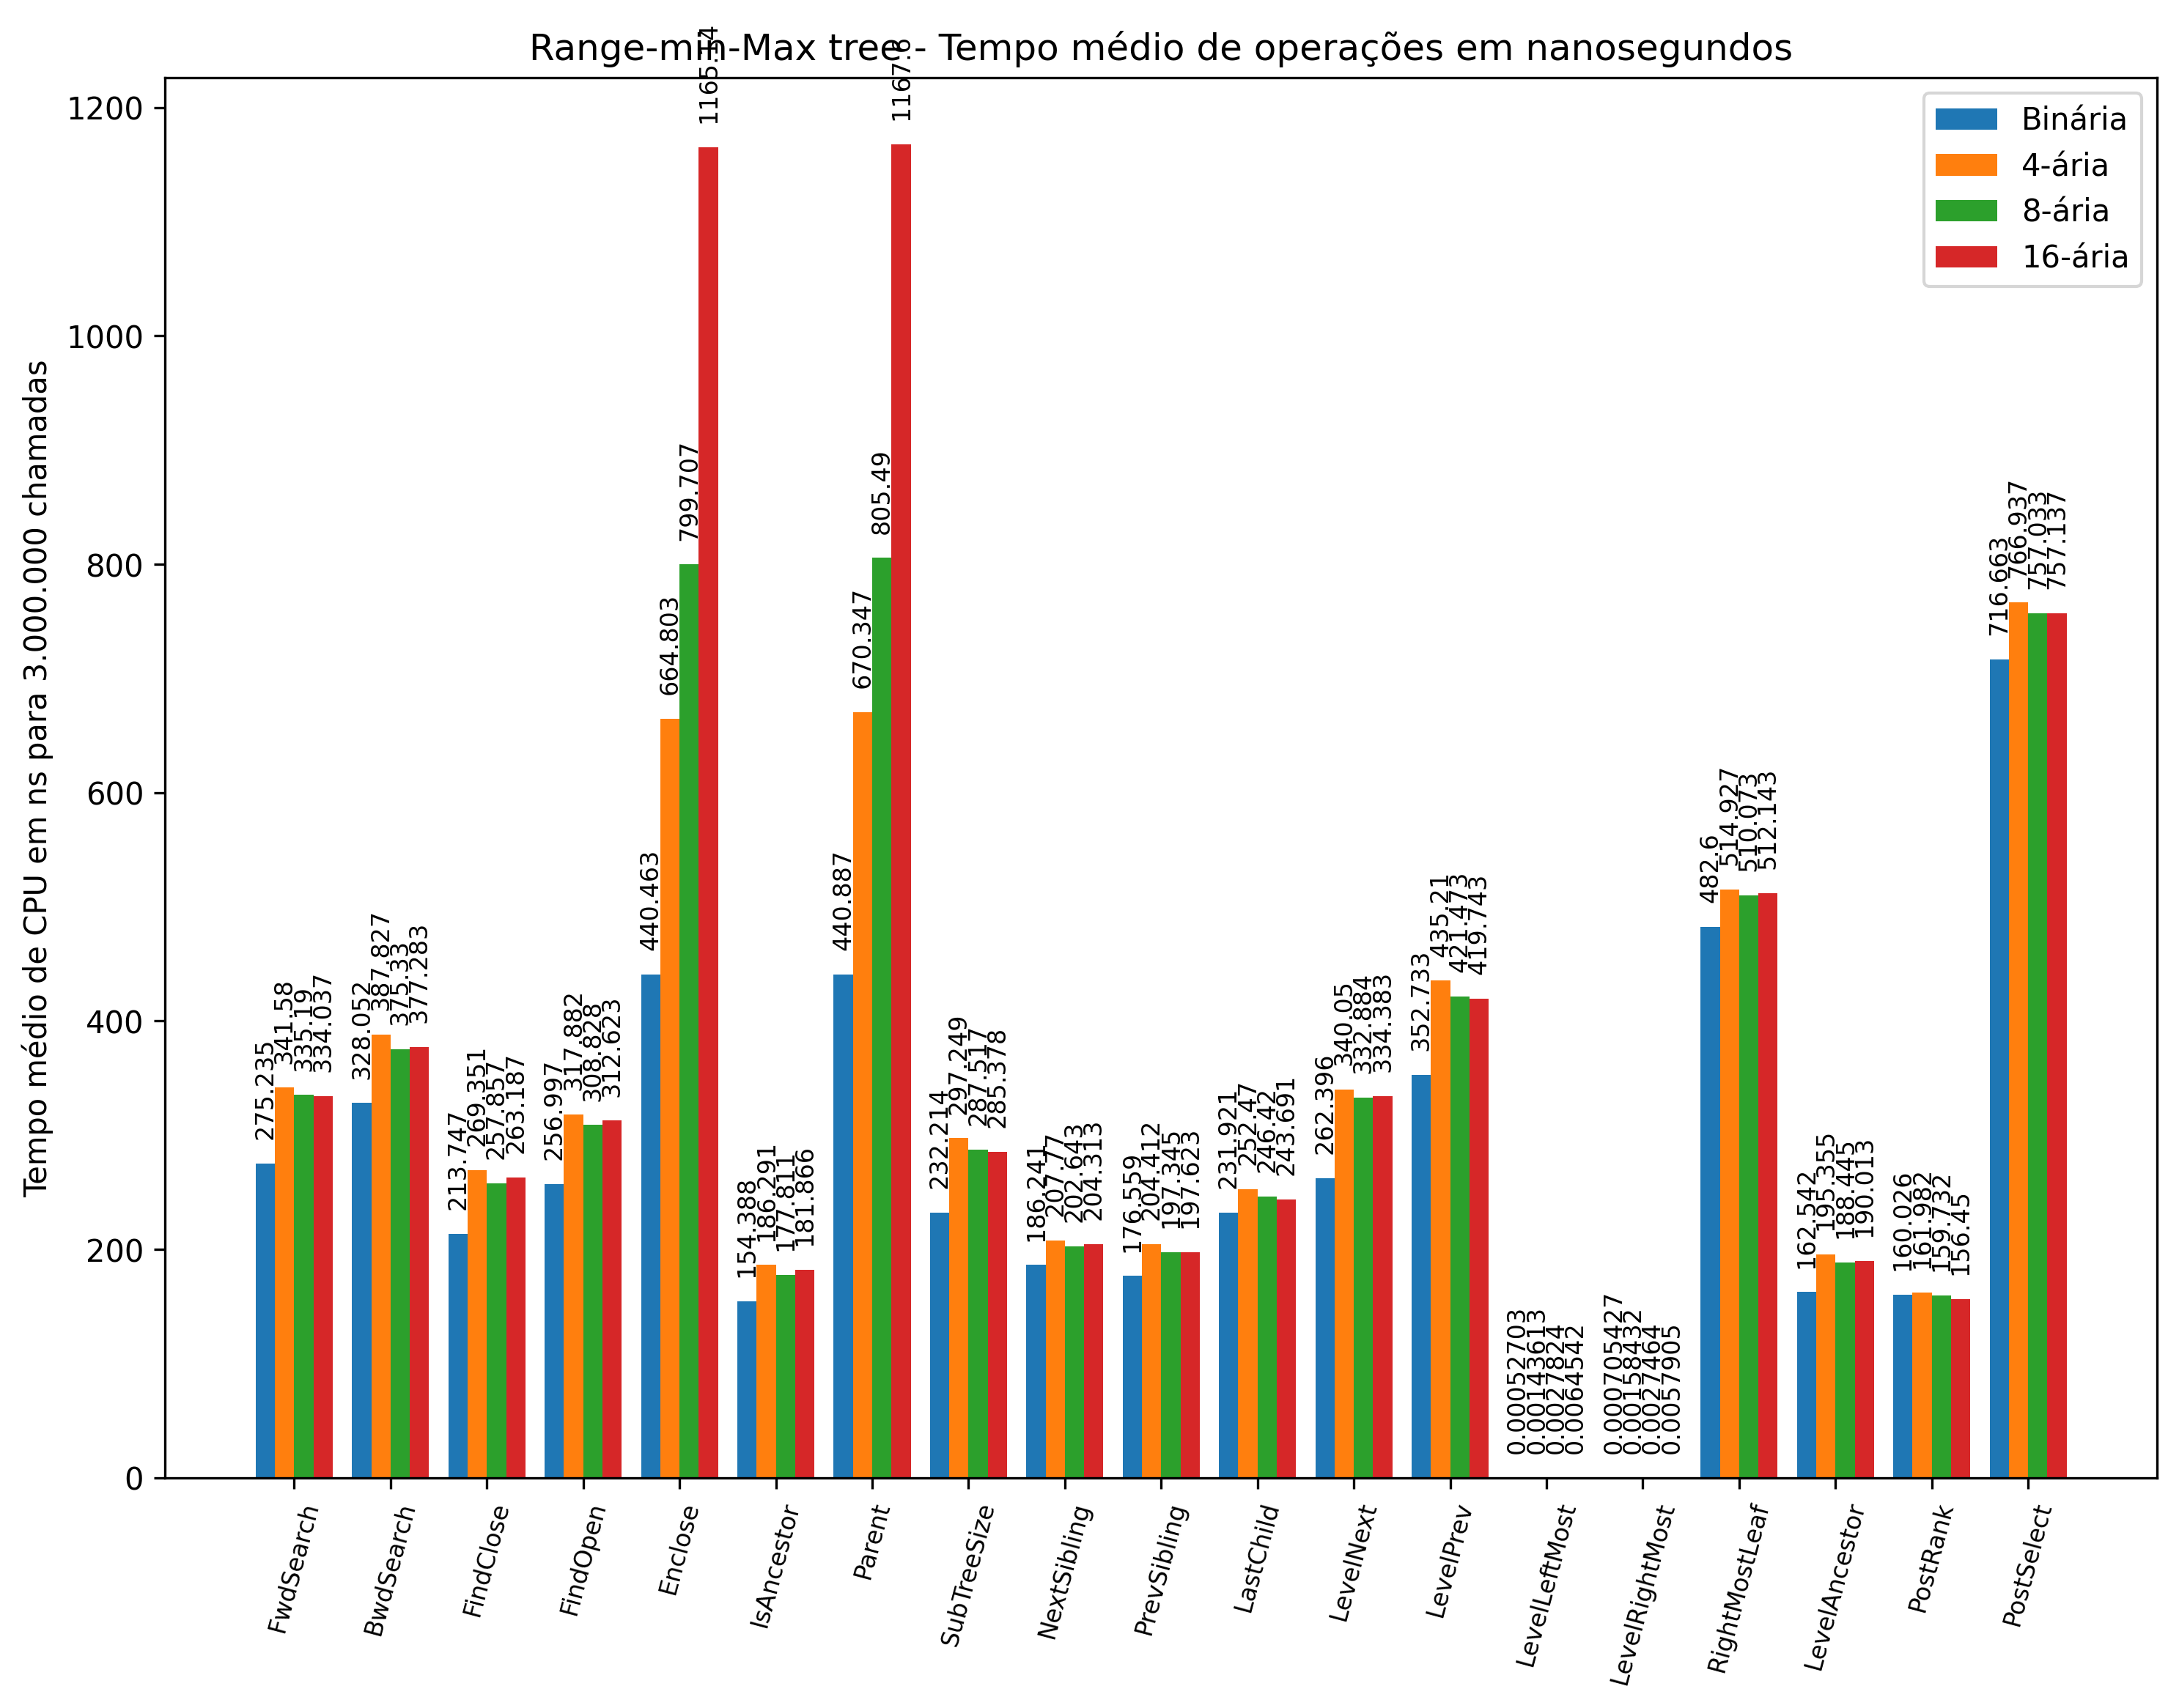
\includegraphics[scale=0.8, angle=270]{images/wiki_i3000000.png}
        }
        \label{fig:wiki}
\end{figure}
%base de dados, configuração, experimentos, resultados
%figura, resultado destacado.